%%
%% Copyright (c) 2018-2019 Weitian LI <liweitianux@sjtu.edu.cn>
%% Creative Commons BY 4.0
%%

\chapter{绪论}
\label{chap:introduction}

%=====================================================================
\section{研究背景和意义}

理解宇宙的起源、结构和演化,是人类孜孜不倦追求的目标,相关探索在哲学和科学中均占据重要地位。
经过几十年的努力,宇宙学的\ac{bbt}终于成为标准模型
\cite{weinberg1972,weinberg2008,peebles1993,peacock1999}。
支持该理论的几个关键证据包括星系的红移--距离关系(即 Hubble 定律)、
\ac{cmb}辐射、星系的大尺度分布规律、早期元素丰度。

根据大爆炸理论,宇宙起源于约 138 亿年前的一次大爆炸。
伴随着宇宙的膨胀,温度和能量密度都逐渐降低,
宇宙依次经历了\ac{inflation}、\ac{bbn}、
\ac{recombination}、\ac{da}、\ac{reionization}、
星系及大尺度结构形成等阶段(如\autoref{fig:univ-history})。

\begin{figure}[htp]
  \centering
  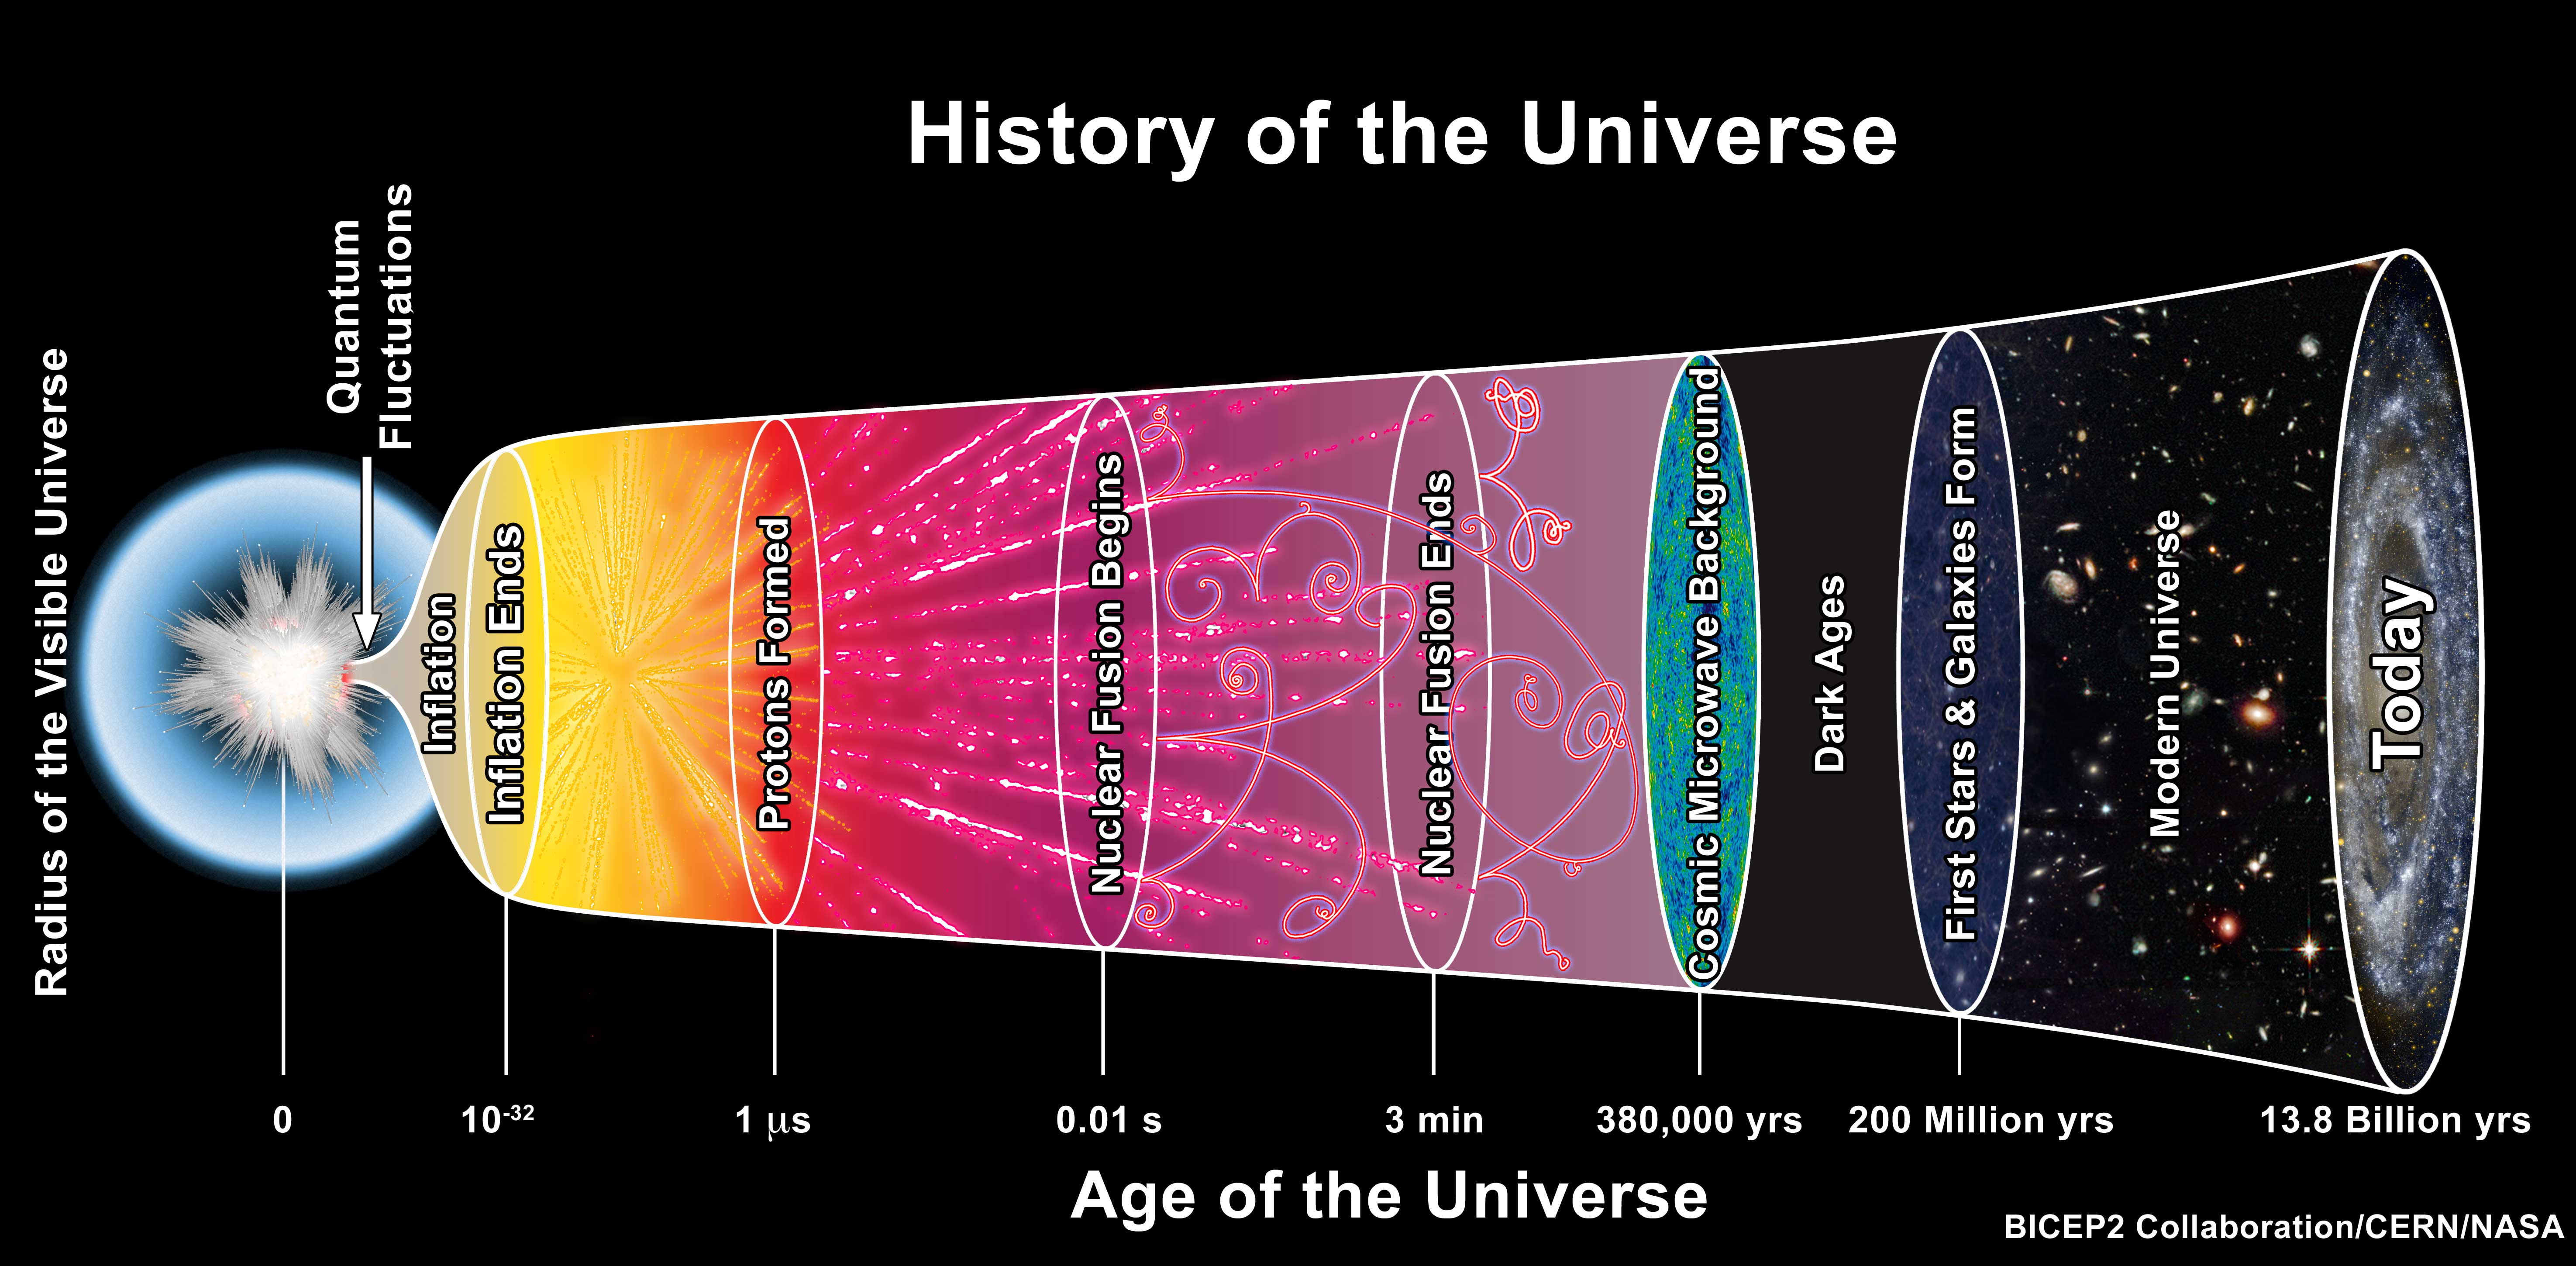
\includegraphics[width=\textwidth]{universe-history}
  \bicaption{%
    宇宙从大爆炸到今天的演化历史
  }{%
    The evolution of the Universe from the Big Bang
    to the present.
    \\来源/Credit:
    \ac{bicep}2/\ac{cern}/\ac{nasa}; \ac{cc}0 1.0
  }
  \label{fig:univ-history}
\end{figure}

大爆炸之后约 40 万年,宇宙冷却至约 \SI{3000}{\kelvin},
自由电子遂与离子结合形成中性原子,于是光子与重子物质脱耦并得以在宇宙中自由传播。
在此时以及之后的一段时间里,第一代恒星和星系尚未形成,因此宇宙进入了\ac{da}。
随着物质的密度扰动在引力作用下增长,第一代天体开始形成并产生辐射,
于是中性重子物质逐步被再次电离,宇宙从此结束\ac{da}并进入\ac{eor}。
随着各尺度上的天体结构的逐步形成与演化,重子物质被充分电离,宇宙形成了今天的格局
\cite{peebles1980,peebles1993,peacock1999}。

通过研究 \ac{cmb},我们对宇宙的极早期历史
($\ac{redshift} \gtrsim 1100$,即自由电子\ac{recombination}之前)有了深刻理解。
另一方面,我们已借助多波段观测掌握了大量有关宇宙近期
($\ac{redshift} \lesssim 6$,即充分电离之后)的演化信息。
然而,我们对 $\ac{redshift} \sim \numrange{6}{1100}$ 那段中间时期却知之甚少。
其中距离相对较近的、红移约为 \numrange{6}{15} 的时期称为 EoR,
从宇宙大爆炸之后约 3 亿年延续到约 10 亿年。
在这个时期,第一代恒星和星系刚形成不久,
辐射的紫外光子和软 X 射线光子使中性重子物质逐渐被再次电离。
针对 EoR 的探测,目前仅能获得非常有限的间接观测信息,
例如,该时期的\ac{hi}对高红移\ac{quasar}的 Lyα 吸收 \cite{becker2001},
自由电子对 \ac{cmb} 光子的 Thomson 散射 \cite{kaplinghat2003}。
但是有关 EoR 的一些关键问题仍然很不清楚,这些问题主要包括:
第一代天体是何时以及如何形成的?
主要的电离源有哪些?它们对再电离过程的贡献分别如何?
\ac{hii}区的尺度以及演化过程如何?
由此可见,EoR 的研究对于理解宇宙早期结构和星系的形成与演化具有重要意义,
是建立完整的宇宙演化图景的关键之一。
详见 \citeay{fan2006}, \citeay{morales2010},
\citeay{pritchard2012}, \citeay{zaroubi2013},
\citeay{koopmans2015}, \citeay{mcQuinn2016} 等综述文。

尽管 EoR 阶段缺乏发光天体可供观测,但是宇宙中充满\ac{hi},
它们辐射的 \ac{21cmline}(详见 \autoref{sec:eor-signal})
为直接探测 EoR 提供了一条可能途径。
事实上,探测\ac{hi} \ac{21cmline}是目前对 EoR 开展系统性研究的最直接而有效的观测手段
\cite{madau1997,tozzi2000,furlanetto2006,koopmans2015,furlanetto2016}。
\ac{hi} \ac{21cmline}的本征频率约为 \SI{1420}{\MHz};
理论预测源自 EoR 的 \ac{21cmline}经历显著红移后应出现在约
\SIrange{90}{200}{\MHz} 之间的低频射电波段。
EoR 信号到达地球时已非常微弱,亮温度仅约几 \si{\mK} 至十几 \si{\mK},
需要具有极高灵敏度的低频观测设备才能开展观测。
目前已建成或正在建设的低频射电干涉阵列主要包括:
\ac{21cma} \cite{zheng2016}、
\ac{gmrt} \cite{paciga2011}、
\ac{mwa} \cite{bowman2013,tingay2013}、
\ac{lofar} \cite{vanHaarlem2013}、
\ac{lwa} \cite{ellingson2009}、
\ac{paper} \cite{parsons2010}、
\ac{hera} \cite{deBoer2017}、
\ac{ska} \cite{mellema2013,koopmans2015}。
必须指出的是,利用干涉阵列探测 EoR 信号面临诸多困难与挑战
\cite{morales2010,wijnholds2010},
例如,如何识别并扣除强烈的前景干扰,如何扣除人工源的\ac{rfi},如何修正电离层的扰动,
如何有效地校准仪器,如何存储并处理海量数据,如何进行高动态范围成像
(详见 \autoref{sec:det-difficulties})。

在低频射电波段,强烈的前景干扰(主要源自银河系以及河外点源;
详见 \autoref{sec:fg-intro})比待探测的 EoR 信号强约 4--5 个数量级,
即便是其涨落也达待测 EoR 信号强度的数千倍 \cite{zaroubi2013}。
从这个意义上讲,准确把握前景干扰并将其扣除是成功探测 EoR 信号的关键。
目前,低频射电波段的观测仍然十分有限,巡天数据严重不足
\cite{deOliveiraCosta2008,zheng2017gal},
导致我们对 EoR 前景的理解程度远远不够
\cite{liu2012,harker2015,offringa2016,murray2017,procopio2017}。
因此,需要挖掘已有中高频射电以及其他波段的海量观测数据,同时结合逐渐积累的低频观测数据,
深入理解 EoR 探测中的低频射电前景并为其构建完善的模型,
为识别和分离 EoR 信号提供有力支撑。


%=====================================================================
\section{研究内容和目标}

EoR 探测涉及诸多重要的科学和技术问题,出于时间和研究条件的考虑,
本文围绕其中关键的 EoR 前景干扰问题开展研究,主要包括以下两个方面的内容:

\begin{itemize}
\item \emph{射电晕辐射建模的改进以及对 EoR 探测影响的评估}

\hspace{2\ccwd}%
深刻理解各前景成分的性质(如强度、空间分布、频谱结构)并充分把握它们对 EoR 探测的干扰方式,
是研发具有针对性的\ac{fg-rm}和 EoR 信号分离算法的前提与关键。
在现阶段缺乏足够可用的高质量低频观测数据的情况下,
借助于挖掘已有多波段观测数据来准确模拟低频射电天空,
是开展前景干扰研究以及 EoR 信号分离算法研发的可行办法。

\hspace{2\ccwd}%
在多种前景成分之中,银河系的弥散辐射 [包括\ac{rad-syn}和\ac{rad-ff}]
以及河外\ac{src-point}辐射是最主要的成分,已被比较广泛地研究过,
它们的低频辐射特征及其对 EoR 探测的干扰行为已经基本被弄清楚
\cite{shaver1999,diMatteo2004,gleser2008,liu2012,murray2017,spinelli2018}。
在剩下的前景辐射之中,来自河外射电\ac{src-extended}的辐射占据主导地位,
主要包括\ac{icm} \cite{feretti2012} 产生的\ac{rh}、\ac{rr}和\ac{rmh},
\ac{gc}外围区域的\ac{igm} 的射电辐射\cite{keshet2004}。
这些河外射电\ac{src-extended}的低频射电观测证据并不多,
尚不明确它们的辐射将如何影响 EoR 信号的探测。

\hspace{2\ccwd}%
与其他几类河外射电\ac{src-extended}相比,星系团\ac{rh}拥有更多的观测数据和理论研究,
使我们有可能构建一个更完善、更物理的模型用来模拟其低频射电辐射特征,
从而改进低频射电天空的模拟,在更加逼真的条件下定量评估不同 EoR 信号探测方法的优劣。

%.......................................
\item \emph{基于深度学习的 EoR 信号分离算法研发}

\hspace{2\ccwd}%
目前已提出一系列方法用来提取淹没于强烈前景干扰之中的微弱 EoR 信号,
这些前景处理方法可大致分为\ac{fg-rm}和\ac{fg-avd}两大类 \cite{chapman2016}
(详见 \autoref{sec:fg-methods})。
前者依赖于一个重要前提:前景辐射的频谱必须非常光滑,可通过构建一个模型来准确地描述。
后者则假定前景干扰被有效地约束在二维\ac{ps}的一个区域内,
于是可以通过尽量避开前景污染区域达到提取 EoR 信号的目标
(详见 \autoref{sec:eor-window})。

\hspace{2\ccwd}%
然而在实际情况中,干涉阵列的\ac{beam}存在频率依赖效应(以下简称波束效应),
即\ac{beam}的形状会随观测频率而变化,导致原本光滑的前景频谱产生快速变化的起伏,
使前景频谱的光滑性遭到损坏 \cite{liu2009ps},
因此现有传统\ac{fg-rm}方法难以区分前景干扰与 EoR 信号,
从而无法正确地分离 EoR 信号(详见 \autoref{sec:beam-effect})。

\hspace{2\ccwd}%
考虑到干涉阵列的\ac{beam}形状非常复杂,为传统前景处理方法打造一个实际可用的模型
用以克服波束效应非常困难 \cite{lochner2015}。
\ac{dl}方法能够从数据中学习特征并自适应地优化模型,
因此基于\ac{dl}的 EoR 信号分离算法能够学习干涉阵列的波束特征,
这将是一条可能的解决问题的途径 \cite{herbel2018,vafaeiSadr2019}。

\end{itemize}

综合上述讨论,我们设定了如下研究目标:
(1) 改进\ac{rh}的模拟,在考虑干涉阵列仪器效应的前提下获得更精细、
更符合实际的低频射电天空的模拟图像,评估\ac{rh}辐射对 EoR 信号探测的影响;
(2) 基于\ac{dl}研发能够有效克服干涉阵列波束效应的 EoR 信号分离新算法,
并运用到上述模拟数据进行测试和优化。


%=====================================================================
\section{研究方案}

本文遵循以下主要步骤开展工作,完成研究内容,达到研究目标:
\begin{enumerate}
\item
调研\ac{rh}的相关理论研究和观测证据,理解其形成机制和演化规律,
构建模型并模拟\ac{rh}在低频射电波段的\ac{skymap}。
搜集\ac{rh}的现有观测数据,约束模型参数,获得可靠的模拟结果。

\item
采用 SKA1-Low 干涉阵列的布局方案,
从上一步所得的\ac{skymap}模拟得到\ac{vis}数据,
然后成像获得高仿真 SKA1-Low 图像。
这种模拟方案可以将干涉阵列的复杂仪器效应(如波束效应)有效地整合到数据分析流程之中。

\item
基于上述模拟所得的 SKA1-Low 图像,利用一维和二维\ac{ps}对比\ac{rh}和 EoR 信号,
量化\ac{rh}辐射在运用\ac{fg-rm}法或\ac{fg-avd}法的情况下对 EoR 信号探测的影响,
评估并研究\ac{rh}干扰的重要性。

\item
从目前主流的\ac{dl}算法中筛选出适用于 EoR 信号分离的算法并加以必要的改善,
利用上述模拟数据对算法进行训练和调优,研究新算法的可行性和优势。

\end{enumerate}


%=====================================================================
\section{本文框架}

本文余下章节安排如下:
\autoref{chap:radio-astronomy}将介绍射电天文学和干涉测量技术的基础知识,
主要包括基本的辐射理论、天线原理、干涉成像技术等。
在\autoref{chap:detection},我们将介绍利用\ac{hi} \ac{21cmline}%
探测 EoR 的基本原理、主要方法、面临的困难、以及前景处理方法。
\autoref{chap:simulation}首先详细描述我们改进的星系团\ac{rh}的建模方法,
然后介绍其他前景成分和 EoR 信号的\ac{skymap}模拟,
最后说明 SKA1-Low 观测图像的模拟。
利用改进的 EoR 前景模型和模拟结果,
我们在\autoref{chap:halo}采用\ac{ps}来评估\ac{rh}辐射对 EoR 信号探测的具体影响,
然后在\autoref{chap:cdae}研究干涉阵列的波束效应对前景辐射频谱光滑性的影响,
接着阐述基于\ac{dl}的 EoR 分离新算法并演示其效果。
最后,我们对全文进行总结并作简要展望。
\autoref{fig:flow-thesis} 显示了本文的主要结构和研究流程。

\begin{figure}[htp]
  \centering
  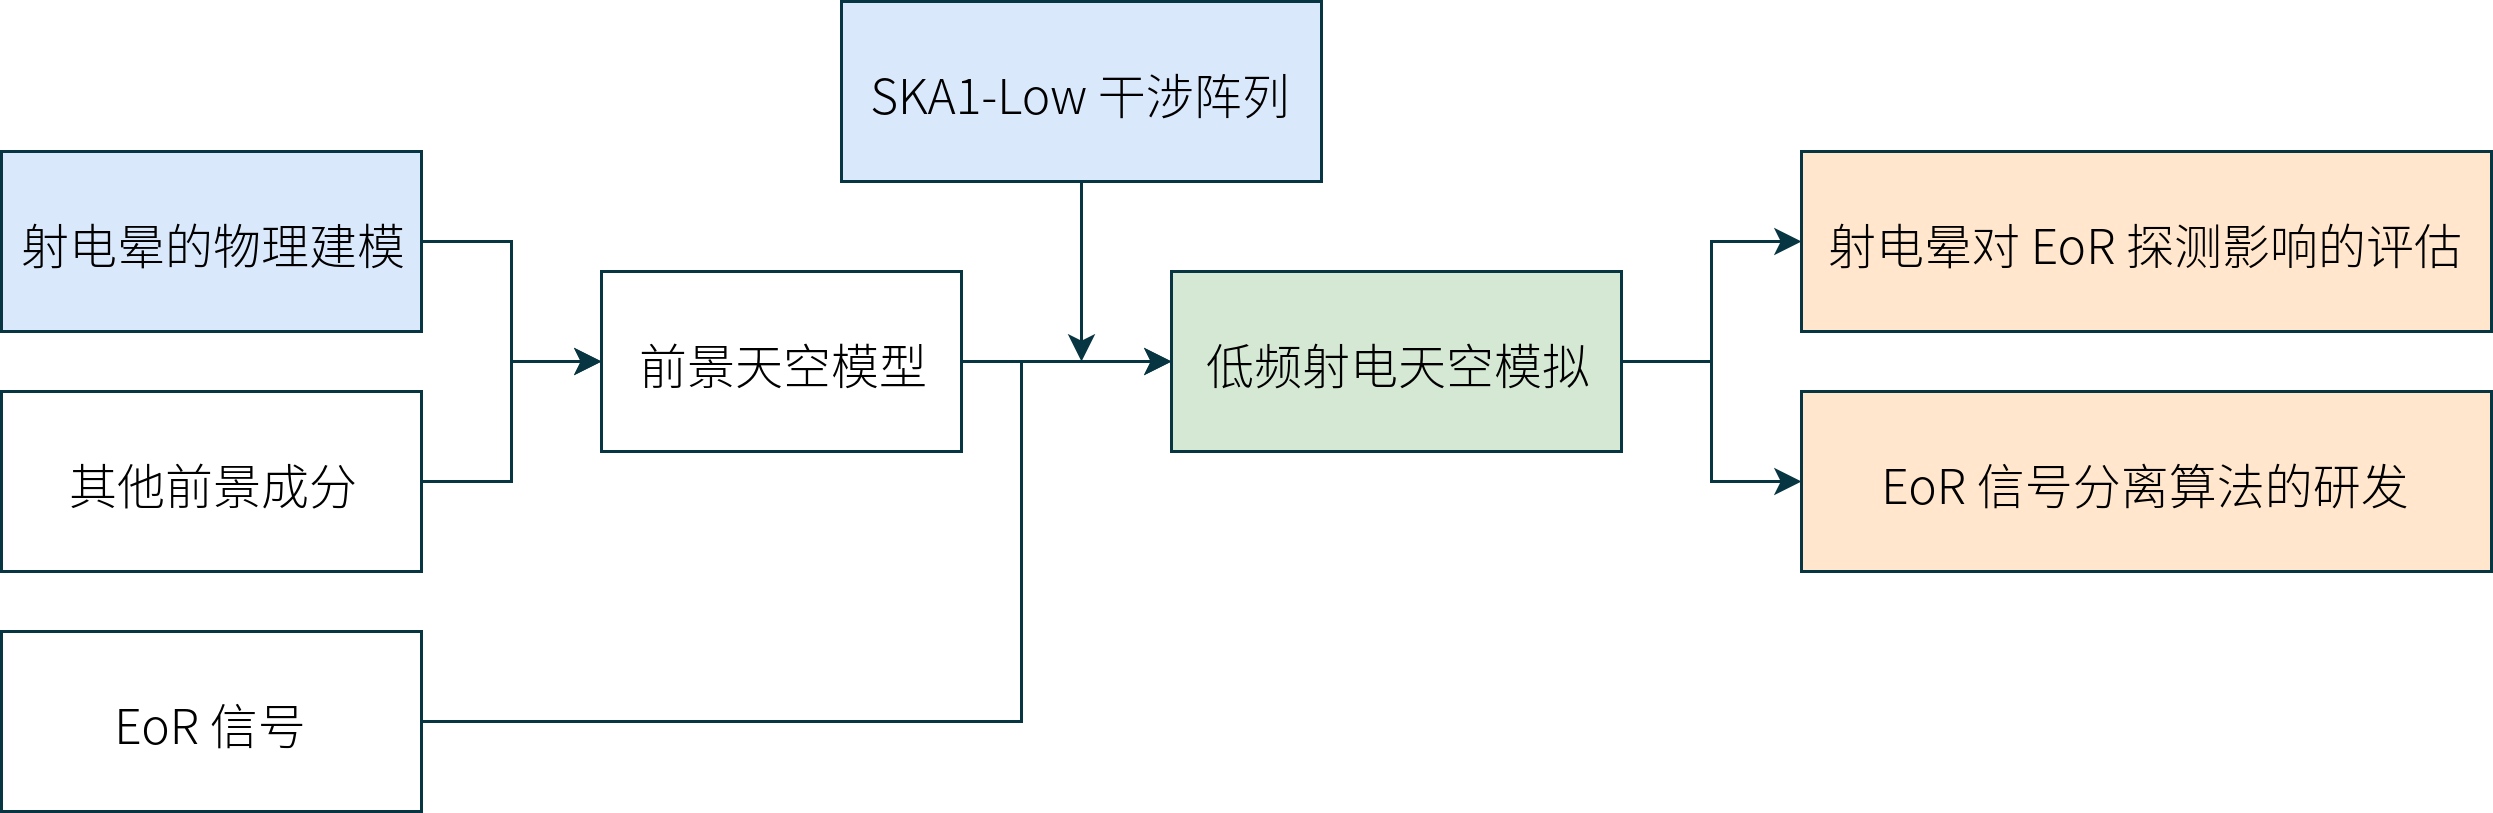
\includegraphics[width=\textwidth]{flow-thesis}
  \bicaption{%
    本文的主要结构和研究流程
  }{%
    The basic structure and the study process of this thesis.
  }
  \label{fig:flow-thesis}
\end{figure}

本文采用一个由 \lcdm 模型描述的平直宇宙,参数为:
$\acs{H0} = 100\,\acs{h}\,\si{\km\per\second\per\Mpc}
= \SI{71}{\km\per\second\per\Mpc}$,
$\acs{Om0} = 0.27$,
$\acs{Ol0} = 1 - \acs{Om0} = 0.73$,
$\acs{Ob0} = 0.046$,
$\acs{ns} = 0.96$ 以及 $\acs{sigma8} = 0.81$。
如无额外说明,本文给出的误差对应 68\% 的置信水平;
使用的幂律谱形式为 $\acs{S-nu} \propto \acs{freq}^{-\acs{spec-index}}$,
其中 \acs{S-nu} 为\acl{S-nu}, \acs{spec-index} 为\acl{spec-index}。
本文使用的中文术语遵循\href{%
  http://astrodict.china-vo.org/
}{英汉天文学名词数据库}\footnote{%
  英汉天文学名词数据库:
  \url{http://astrodict.china-vo.org/}}
以及 Google 的\href{%
  https://developers.google.com/machine-learning/glossary/?hl=zh-CN
}{机器学习术语表}\footnote{%
  机器学习术语表:
  \url{https://developers.google.com/machine-learning/glossary/?hl=zh-CN}}。


%% EOF
